\documentclass[10pt,a4paper]{article}
\usepackage[utf8]{inputenc}
\usepackage{amsmath}
\usepackage{amsfonts}
\usepackage{amssymb}
\usepackage{amsthm}
%\usepackage{mathrsfs}
\author{Dylan Swiggett}
\title{Image Matting and Applications}

\begin{document}
\maketitle

\begin{abstract}
Image matting is a practical and heavily applied technique in image recognition, useful both on its own and as an intermediate stage in image and video processing. In this paper, I explain the basics of image matting theory, then discuss several specific techniques documented in \textit{Scalable Matting: A Sub-linear Approach} \cite{lee14}. I conclude with a few applications of the techniques described, and demonstrate some results of my own implementation.
\end{abstract}

\tableofcontents
\pagebreak

% Add blank page 2 for printing.
\iffalse
\pagestyle{empty}
\begin{quote}
\item
\end{quote}
\pagebreak
\setcounter{page}{2}
\pagestyle{plain}
\fi

\section{Introduction}
\subsection{Image Matting}
Image matting is an extensive field, but in this paper I focus on foreground and background extraction. Given an image $I$, we wish to produce a \textbf{matte} (a trasparency value $\alpha$ at each pixel, with $\alpha_{i}\in[0,1]$) such that at each pixel $i$ we can deconstruct the color value $I_{i}$ into a sum of two samples, one from a foreground color $F_{i}$ and one from a background color $B_{i}$. To produce the color value at each pixel $i$ in our original image, we then take
\[I_{i}=\alpha_{i}F_{i}+(1-\alpha_{i})B_{i}\]
This problem is constrained with a ``sketch" by the user, often called a \textbf{prior}, indicating regions of the image which are known to be either in the foreground or in the background. With enough such constraints, the problem can be sufficiently defined such that an accurate and useful matte is produced.
\subsection{Topics Covered}
\textit{Scalable Matting: A Sub-linear Approach}, by Philip G. Lee and Ying Wu, documents the steps of several modern image matting techniques, and compares them both analytically and practically. Lee and Wu provide a few different methods for each step of the matting algorithm, bit in this paper I focus in on specific examples. I give brief explanations of most algorithms tested, and focus in particular on the Matting Laplacian from \cite{levin08} and the V-Cycle algorithm detailed in \cite{briggs87} and \cite{bramble93}. I then give previews of a few of the applications of this method, before concluding with some experiments performed with my own implementation.
\section{Definitions}
\subsection{Graph Laplacian}
We have a non-looping, unweighted, and undirected graph. We take $v_i$ to be an indexing of its vertices.
We first define the \textbf{degree matrix} of our graph, $D$, to be a diagonal matrix where $D_{ii}$ is the degree of $v_i$ (the number of adjacent edges).
Next, we define the \textbf{adjacency matrix} of our graph, $A$, a symmetric matrix where $A_{ij}=1$ iff there is an edge between $v_i$ and $v_j$. Note that, since our graph is non-looping, $A_{ii}=0$.
The \textbf{Graph Laplacian}, $L$, of our graph is now defined as $L=D-A$ \cite{weisstein}.
\subsection{Matting Laplacian}
When dealing with image matting, we can construct a graph such that each pixel is a vertex and adjacent pixels share an edge. Such a graph is naturally undirected and non-looping. However, the bulk of image matting is determining appropriate weights for the edges, so we cannot immediately construct a Graph Laplacian. Instead, we use a variant of the Graph Laplacian called the \textbf{Matting Laplacian} \cite{levin08}. Although identical in construction, our $D$ and $W$ must be produced through a different vertex \textbf{affinity function} than simple adjacency. The choice of this affinity function is open, but we use the form shown in \cite{levin08}, which is outlined in \textbf{Techniques}.
\\\\
In general, we can solve for our values of $\alpha$ by minimizing the quadratic form
\[J(\alpha)=\alpha^T L\alpha\]
\textbf{I will explain why this is, in the final draft.} One of the key properties of a matting Laplacian is that it is positive semi-definite, so can be minimized to a non-trivial solution by solving a system of linear equations. The majority of this paper is devoted to methods for efficiently solving this system of equations for any given Matting Laplacian.
\subsection{Iterative Methods and Relaxation}
A common problem in computation, and one we will have to address for foreground/background matting, is the solution of large systems of linear equations. We denote these as in \cite{briggs87} by
\[A\textbf{u}=\textbf{f}\]
As shown later, the systems of linear equations involved are massive for even reasonably sized images, and although direct solutions are possible, they are difficult to approach both in theory \cite[pg.4]{briggs87} and in practice \cite{lee14}. Instead, we take an iterative approach. We take an approximation of $\textbf{u}$, denoted $\textbf{v}$. This approximation might be initially very rough, but through successive iterations our approximation should converge towards $\textbf{u}$. To formalize this, we define the \textbf{error} ($\textbf{e}$) and the \textbf{residual} ($\textbf{r}$) by
\[\textbf{e}=\textbf{u}-\textbf{v}\hspace{.5in}
  \textbf{r}=\textbf{f}-A\textbf{v}\]
We then note that, in combination with our original system of equations, we have that
\[A\textbf{e}=\textbf{r}\]
This is known as the \textbf{residual equation} \cite{briggs87}. While the error is not immediately available unless the system of equations is already solved, the residual can be calculated at any intermediate step, so this gives us a first clue as to how an iterative step might be produced:
\[\textbf{u}=\textbf{v}+\textbf{e}=
	\textbf{v}+A^{-1}\textbf{r}\]
Since $A^{-1}$ is usually very difficult to compute, the first step in \textbf{relaxation} (the general name for these iterative solutions) is to find some similar matrix. We denote the residual and approximate solution after $n$ steps by $\textbf{r}^{(n)}$ and $\textbf{v}^{(n)}$, and rephrase our goal as finding a $B\approx A^{-1}$ or a matrix $P$ and a vector $\textbf{g}$ such that
\[\textbf{v}^{(n+1)}=\textbf{v}^{(n)}+B\textbf{r}^{(n)}
	=P\textbf{v}^{(n)}+\textbf{g},
\hspace{.5in}
	\lim\limits_{n\to\infty}
		\left\Vert\textbf{r}\right\Vert^{(n)}=
	\lim\limits_{n\to\infty}
	\left\Vert\textbf{e}\right\Vert^{(n)}=0\]
These notations are mathematically equivalent, but going forward we will use the $P$ and $\textbf{g}$ notation. Now, we can see that if some solution $\textbf{u}$ does exist, it satisfies
\[\textbf{u}=P\textbf{u}+\textbf{g}\]
So we have that
\[\textbf{e}^{(1)}=\textbf{u}-\textbf{v}^{(1)}
=(P\textbf{u}+\textbf{g})-(P\textbf{v}^{(0)}+\textbf{g})
=P\textbf{e}^{(0)}\]
Extending this through multiple iterations,
\[\textbf{e}^{(n)}=P^n\textbf{e}^{(0)}\hspace{.5in}
\left\Vert\textbf{e}^{(n)}\right\Vert\leq
\left\Vert P\right\Vert^n
	\left\Vert\textbf{e}^{(0)}\right\Vert\]
So our constraint to guarantee convergence is that the \textbf{spectral radius} of $P$ (the maximum norm of its eigenvectors) is less than $1$. We will demonstrate an example for which this is true in \textbf{Techniques}.
\subsection{Multigrid Methods}
Multigrid methods were invented as a solution to poor convergence behavior on low frequency error components. The idea is to downsample the system of linear equations, such that the low frequency modes which occur at high resolution become high frequency modes at coarse resolution, and hence converge quickly. Fortunately, the mathematical basis built up for our system of equations translates well into this framework. We refer back to the notation used in the interpolation section, $\textbf{v}^h$ referring to $\textbf{v}$ at resolution $h$, as this notation is used extensively in this section.
\\\\
The general algorithm for a multigrid is to produce a high resolution error, then downsample it, correct as much error as possible (through iteration) at this coarse level, then upsample and apply the error corrections to the higher level of detail. Naively, we can summarize this as starting with a good $\textbf{v}^h$ by first solving (or approximating) $\textbf{v}^{16h}$ or some variant, then applying our interpolation operator several times to produce our more detailed error. Unfortunately, this simple algorithm is not easy to apply when we are given an initial guess, $\textbf{v}^{(0)}$, at the highest level of resolution. However, the residual equation here comes to the rescue:
\[A\textbf{e}=\textbf{r}\hspace{.5in} A^{h}\textbf{e}^{h}=\textbf{r}^{h}\]
Our $A^{h}$ and $\textbf{r}^{h}$ are known, and the initial guess for $\textbf{e}^{h}$ is $\textbf{0}$, regardless of the $\textbf{v}^{(0)}$ chosen. Further, this is yet another system of linear equations, involving smaller values, and with a simpler convergent case. This leads us to the first candidate for a multigrid algorithm:
\vspace{-.2in}
\begin{quote}
\item
\subparagraph{Nested Iteration \cite{lee14}}
\begin{enumerate}
\item Calculate $r^h$ from $f^h-A^h{v}^{(n)h}$\\
(note that $\textbf{v}^{(n)h}$ is a combination of notations $\textbf{v}^{(n)}$ and $\textbf{v}^h$).
\item Calculate $r^{2h}$ from the restriction operation $I_{h}^{2h}r^h$.
\item Solve $A^{2h}\textbf{e}^{2h}=r^{2h}$ for $\textbf{e}^{2h}$ by Nested Iteration with $\textbf{e}^{(0)2h}=0$.
\item Calculate $\textbf{v}^{(n+1)h}$ from
	$\textbf{v}^{(n)h}+I_{2h}^he^{2h}$
\end{enumerate}
\end{quote}
\vspace{.2in}
This method is quite effective, but only if the error is relatively smooth. Namely, the interpolation operation at the final step must make a good approximation of the actual error. However, we now have an algorithm that preserves corrections to smooth error but not oscillatory error. Clearly, combining this with a relaxation method such as Gauss-Seidel could have good results.
\\\\
This combination leads to what is known as the \textbf{V-Cycle Method}, so called for the V-like shape in which it first restricts repeately, then interpolates repeatedly. Following is the pseudocode for this algorithm in \cite{lee14}:
\vspace{-.2in}
\begin{quote}
\item
\pagebreak
\subparagraph{V-Cycle Pseuodocode}
\begin{enumerate}
\item[1:] function VCYCLE$_H$($\textbf{u}^h$,$f^h$):
\item[2:] \hspace{.2in} if $h=H$:
\item[3:] \hspace{.4in} return final solution $\textbf{u}^h$
\item[4:] \hspace{.2in} Relax on $A^h\textbf{u}^h=f^h$
\item[5:] \hspace{.2in} $r^{h}\leftarrow f^h-
						A^h\textbf{u}^h$
\item[6:] \hspace{.2in} $\textbf{e}^{2h}\leftarrow$
						VCYCLE$_H(\textbf{e}^{2h}=0,
						I_h^{2h}r^h)$
\item[7:] \hspace{.2in} $\textbf{u}_h\leftarrow
						\textbf{u}^h+I_{2h}^h
						\textbf{e}^{2h}$
\item[8:] \hspace{.2in} Relax on $A^h\textbf{u}^h=f^h$
\item[9:] \hspace{.2in} return $\textbf{u}^h$
\end{enumerate}
\end{quote}
\vspace{.2in}
In fact, this algorithm is guaranteed to converge in a fixed number of iterations (conditioned on $n^2$) \cite{gopal08}.
\section{Techniques}
\subsection{Example Matting Laplacian}
I here outline the Matting Laplacian (and derivation) performed in \cite{levin08}. Although many alternate (and often simpler) affinity functions are documented, this one is both common and rigorous. This solution makes a few small simplifying assumption. The first is that the foreground and background images are locally smooth. This leads to sudden changes in the image color being attributed to sudden changes in $\alpha$, a reasonable expectation. The second is that the image is greyscale, which significantly simplifies calculations and can be worked around later. Given this second assumption, greyscale values will throughout this paper be treated as bounded real numbers.
\\\\
From the smoothness assumption, we can locally treat our values of $\alpha$ as a linear function, conditioned on known values for $F$ and $B$, the foreground and background images. Taking $a=\frac{1}{F-B}$ and $b=-\frac{B}{F-B}$, we define our matte by
\[\alpha_i=aI_i+b\]
for all values of $i$ in a small section of the image. These values of $a$ and $b$ can be justified by noting that $I_i\in[B_i,F_i]$, and the chosen $a$ and $b$ produce $\alpha_i:\,[B_i,F_i]\to[0,1]$, as expected.
\\\\
Solving for $F$ and $B$ is now equivalent to solving for $a$ and $b$. This is done by minimizing a cost function that is chosen in \cite{levin08} to be
\[J(\alpha,a,b)=
	\sum_{j\in I}\left(\sum_{i\in w_j}\left(
		\alpha_i-a_jI_i-b_j\right)^2+\epsilon
		a_j^2\right)\]
with $w_j$ a small box around the pixel $j$. The last term of the sum serves to minimize $a_j$ where possible, and acts to both smooth the matte as a whole, and to resolve convergence where results might otherwise be indeterminate (e.g. a box where the image color is constant). Since the minimal values in each box are determinate, and since they overlap at nearby pixels, this cost function allows local changes to propogate through their neighbors. Cost minimization is solved in \cite{levin08} as follows.

\newtheorem{matlapthm}{Theorem}
\begin{matlapthm}
\end{matlapthm}
\begin{proof}
\end{proof}
\subsection{The V-Cycle Algorithm}
\section{Applications}
While image matting for foreground and background is useful as a standalone technique in image processing, it has garnered significant attention from researchers due to its far-reaching applications in other areas of graphics study. Several of these applications are discussed here.

\subsection{Dehazing}
Image dehazing and its similarities to image matting are explored in detail by \cite{he11}. The basic problem is that, in images taken over some distance, floating particles and moisture can lead to dulling of color for more distant objects. This can significantly reduce the quality of the image taken. Dehazing attempts to determine how much this ``haze" has altered the color at each pixel of an image, and to restore the color to what it would have been if unobscured. The general statement of the problem is to find a solution of the form
\[I_i = J_it_i+A_i(1-t_i)\]
As in image matting, $I$ is the color value at each pixel of the original image, and $t$ is a transparency value at each pixel. In the case of dehazing, $t$ is referred to as the \textbf{medium transmission}, specifying how much of the light from the original source reaches the camera without being scattered by ambient particles. $J$ is the color of the desired image at each pixel, referred to as the \textbf{scene radiance}, while $A$ is global atmospheric light.
\\\\
A prior for this problem is produced by noting the existence of a so-called \textbf{dark channel}. \cite{he11} observes from a set of haze-free daytime images that natural images almost always have at least one color channel (red, green, or blue) close to zero at every pixel. In contrast, the ambient light in images with haze increases every pixel's color value uniformly, preventing the existence of a dark channel where significant haze occurs.
\subsection{Deblurring}
In images taken of moving scenes, objects that move a visible distance during the image exposure have visible blur along the direction in which they move. In \cite{dai08}, this blur is both removed, and analyzed to determine how objects in a single picture were moving when the picture was taken. The key innovation of \cite{dai08} is to begin analyzing motion blur by matting the image for alpha (exactly as described in this paper) in order to determine how much a given object has blurred into each pixel. See \cite{dai08} for further details, as beyond this initial step matting is unrelated to deblurring.
\subsection{Tracking}
A common problem in video analysis is to track a specific object over a period of time. The relationship between this and image matting is immediately apparent, in that both techniques aim to determine which part of an image is a specific object. The key difference is that in image matting, a user must give constraints, whereas in tracking the goal is to automatically determine which part of a frame is the object given only the same knowledge for the previous frames. This issue is overcome in \cite{fan10} by building model of the object being tracked, kicked off by actual user constraints on the first frame. This is then used it to produce a ``user sketch" entirely programmatically at each subsequent frame, before applying the standard image matting algorithm.
\\\\
The model of the object generated is divided into three major components. First, a set of \textbf{salient points} (points recognizable as lying inside the object) are generated. A sketch can be produced by drawing lines between these salient points. However, as an object moves or deforms, these points can quickly become unrecognizable by simple algorithms. As such they are generated as the program goes on, and are a purely short-term part of the model. Next, a set of \textbf{discriminative colors} are selected. These are specific colors which occur far more frequently in either the foreground or the background, and are generally a much better long-term indicator of where a given object lies. However, they are also updated as frames are processed, since new parts of an object might become visible. Finally, the region of the image known to be foreground is cut up into square regions, and each of these regions is stored individually in a \textbf{bag of patches}. At each frame, each patch is checked against the contents of the scene. If some patch is found to be unobscured, it is assumed to be part of the foreground. These patches are the most long-term model of the object, and can be used to determine new salient points even when the tracked object is severely occluded (i.e. something passes in front of it) or deformed.
\\\\
With these three models, each of which is sequentially updated by methods described in \cite{fan10}, a sufficiently accurate and dense user sketch can be generated to apply image matting effectively at each frame. The results far outperform more traditional video matting techniques for tracking.
\section{Experiments}
In order to better understand the algorithm, and to test its effectiveness, I created my own implementation. I used \textbf{Successive Over-Relaxation} as opposed to Gauss-Seidel, since this exhibited better results (SOR is the same as Gauss-Seidel, except that after solving for the error and interpolating, the result is multiplied by a user chosen value between 0 and 2). I also used a variant on the Matting Laplacian from \cite{levin08} that takes into account the RGB channels of the image, rather than just the grayscale intensity at each pixel. I used the interpolation and restriction operators described in \cite{lee14}, as well as the V-Cycle algorithm for multigrid. Since speed was an important factor in testing my implementation, I chose to write it in C++ (a decision made also by the authors of \cite{lee14}).
\\\\
In general, my results were quite impressive. My implementation does not exhibit convergence as rapidly as \cite{lee14}, so I believe there may still be errors in the code, but this does not prevent most images from converging to fairly accurate mattes. One of the most prominent features of this method is just how much of a different the multigrid optimization makes. Consider the following image and sketch:
\\
\begin{center}
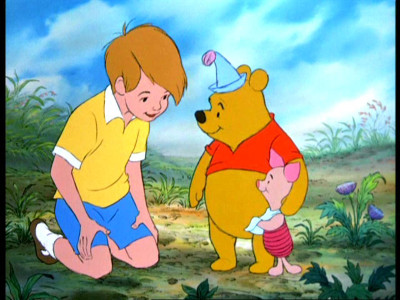
\includegraphics[width=2.2in]{fig/pooh_med.jpg}
\hspace{.2in}
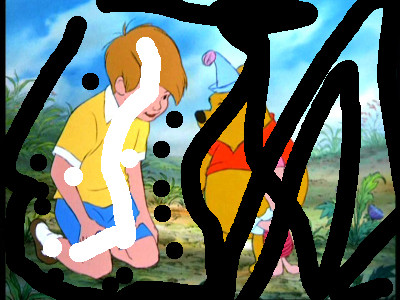
\includegraphics[width=2.2in]{fig/christopher_med_sketch.jpg}
\end{center}
The following images were both produced with 50 iterations of SOR, but the first did not have multigrid steps enabled, while the second did. The difference is startling!
\\
\begin{center}
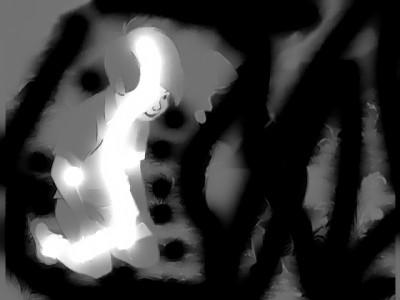
\includegraphics[width=2.2in]{fig/christopher_med_result_nogrid.jpg}
\hspace{.2in}
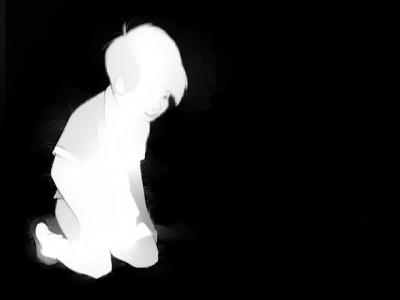
\includegraphics[width=2.2in]{fig/christopher_med_result.jpg}
\end{center}
This difference is just as pronounced on other images. Clearly relaxation has similar problems on images as it did on the sample problem earlier explained! In the second image, it's apparent that there are issues with matting around the edges of the image. Although this is likely mostly an implementation issue, I did notice that many of the images shown in papers used images with in-focus foregrounds and blurry, relatively uniform backgrounds. When applied to images of this type, my implementation also had quite impressive results. With 30 iterations, the following sketch produced an excellent matte:
\\
\begin{center}
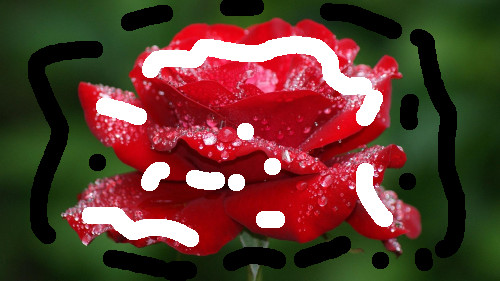
\includegraphics[width=2.2in]{fig/rose.jpg}
\hspace{.2in}
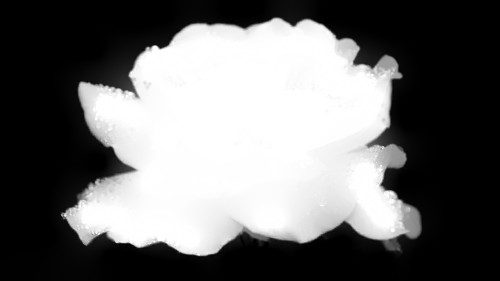
\includegraphics[width=2.2in]{fig/rose_result.jpg}
\end{center}
In instances such as this, the practical applications of image matting in simple image editing become quite apparent. Complex shapes can be cut out of images with minimal effort and high accuracy. When results are not satisfactory, adding a few lines to the sketch is almost always sufficient. For example, the above matte was used to produce the image below.
\\
\begin{center}
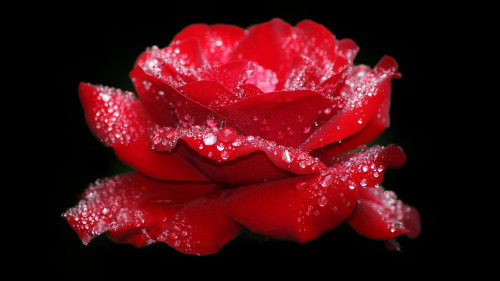
\includegraphics[width=4.6in]{fig/rose_blackbg.jpg}
\end{center}
With a bit of effort to produce a good sketch, very good mattes can be produced. However, one drawback of the strict constraints of the user sketch can become apparent on images with large semi-transparent regions. Consider the following matting application:
\\
\begin{center}
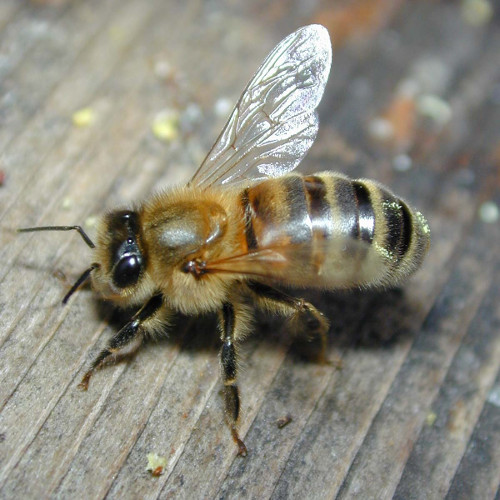
\includegraphics[width=2.2in]{fig/bee.jpg}
\hspace{.2in}
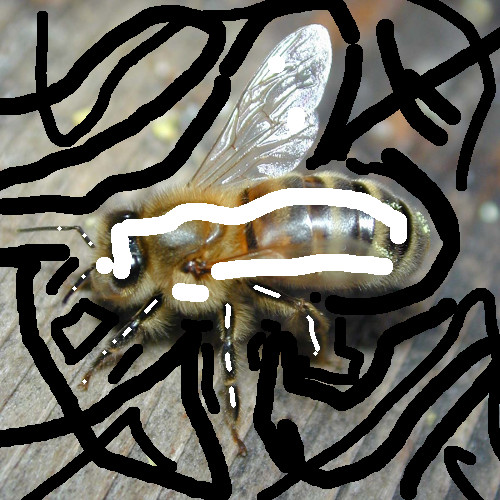
\includegraphics[width=2.2in]{fig/bee_sketch.jpg}
\end{center}
\begin{center}
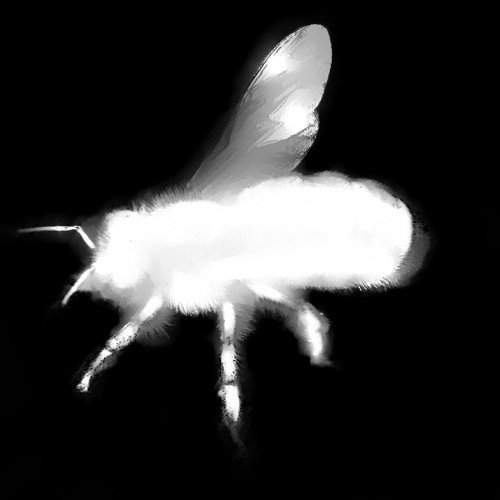
\includegraphics[width=2.2in]{fig/bee_result.jpg}
\hspace{.2in}
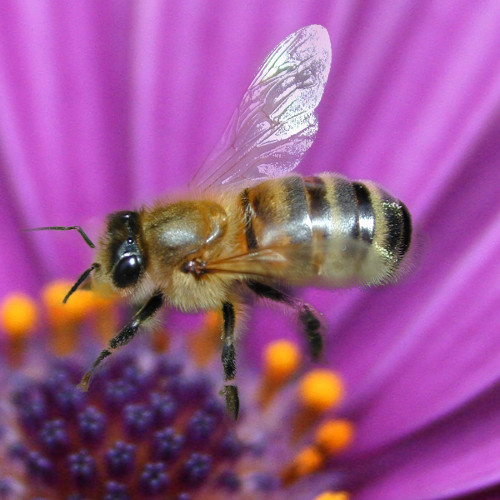
\includegraphics[width=2.2in]{fig/bee_on_flower.jpg}
\end{center}
The complex shape of the bee is selected very accurately withe the sketch given, but the wings are a problem. They are everywhere transparent, but any places marked as part of the foreground then become complete opaque. In the above matte, it is clear that the correct transparency was determined for most of the wing, but the places marked in the sketch are unnaturally white.
\\\\
The code for this implementation can be found at\\ \url{https://github.com/dylanswiggett/image-matting/tree/master/impl}.

\pagebreak
\textbf{Fill this stuff out:}

\begin{thebibliography}{9}
\bibitem{lee14}
	Philip G. Lee, Ying Wu,
	``Scalable Matting: A Sub-linear Approach."
	
\bibitem{levin08}
	Anat Levin et al,
	``A Closed Form Solution to Natural Image Matting."
	
\bibitem{weisstein}
	 Weisstein, Eric W. "Laplacian Matrix." From 	\textit{MathWorld}--A Wolfram Web Resource. http://mathworld.wolfram.com/LaplacianMatrix.html 
	 
\bibitem{briggs87}
	William L. Briggs, \textit{A Multigrid Tutorial},
	Society for Industrial and Applied Mathematics, 1987.
	
\bibitem{bramble93}
	James H. Bramble, \textit{Multigrid methods},
	Longman Scientific \& Technical, 1993.
	
\bibitem{gopal08}
	J. Gopalakrishnan and J. E. Pasciak,
	``Multigrid convergence for
second order elliptic problems with smooth complex coefficients."

\end{thebibliography}
\end{document}